% =====================================================================
%  Capítulo 8 — Resultados
% =====================================================================
\chapter{Resultados}
\label{cap:resultados}
\rubricaComunicacao

\section{O sistema em operação}

A Figura~\ref{fig:resultado} mostra a campanha inteira: temperatura,
umidade e luz, com o mesmo eixo de tempo. A linha é interrompida em toda
lacuna maior que \SI{450}{\second} (1,5 período), sem interpolação; as
faixas cinzas marcam as lacunas e as linhas tracejadas vermelhas, os
reinícios do nó. A figura é gerada por \caminho{dados/grafico.py} a partir
de \caminho{dados/mensagens_limpo.csv}.

\begin{figure}[H]
\centering
\IfFileExists{figuras/serie-campanha.pdf}{%
  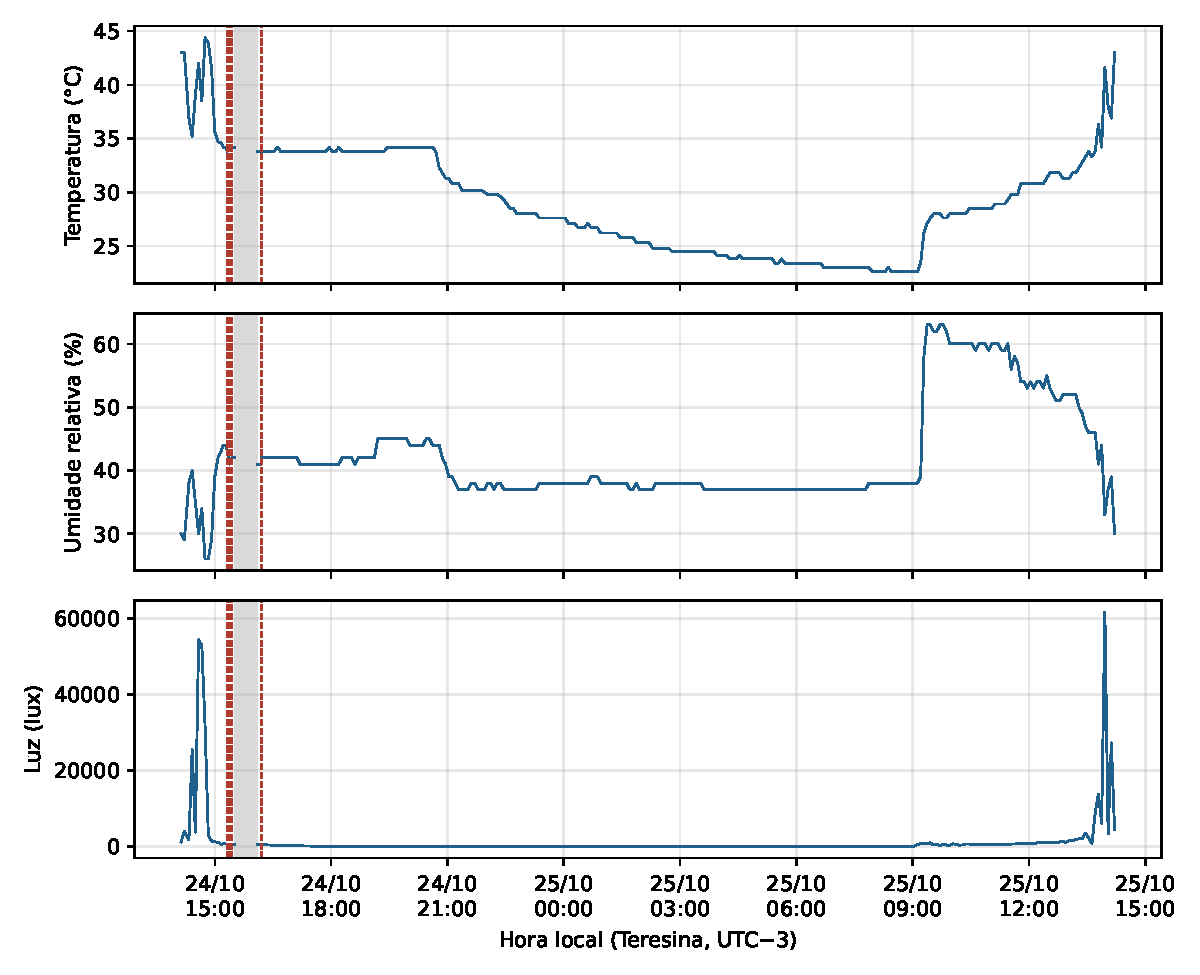
\includegraphics[width=\textwidth]{figuras/serie-campanha.pdf}}{%
  \fbox{\parbox[c][5cm][c]{0.9\textwidth}{\centering\small
    figura ausente: gerar com \texttt{dados/grafico.py}}}}
\caption{Temperatura, umidade relativa e luz durante a campanha, com as lacunas à vista}
\label{fig:resultado}
\fonte{Dados coletados pela equipe de 24/10/2026, 14:07, a 25/10/2026, 14:13.}
\end{figure}

\noindent O que a série mostra:
\begin{itemize}
  \item \textbf{Ciclo diário:} a luz e a temperatura têm pico perto das 14\,h
    nos dois dias, quando o sol entra direto pela janela; a máxima foi de
    \SI{44.4}{\celsius} às 14:44 de 24/10 e a mínima, de
    \SI{22.6}{\celsius}, às 07:57 de 25/10, com o ar-condicionado ligado
    desde as 20:34. A amplitude foi de \SI{21.8}{\celsius} e de 37 pontos
    de UR (26 a 63\,\%). Parte dela não é do ambiente: ao sol direto, o
    DHT11 aquece, e as máximas acima de \SI{40}{\celsius} são do sensor
    aquecido.
  \item \textbf{Luz:} máximo de \SI{61571}{lux} às 13:57 de 25/10; acima de
    \SI{20000}{lux} só em 6 leituras, entre 14:24 e 14:44 de 24/10 e
    entre 13:57 e 14:07 de 25/10. Nenhum dia de calendário ficou
    completo; as 24,1\,h somaram cerca de \SI{2.0}{\mol\per\square\metre}
    (1,06 em 24/10, das 14:07 à meia-noite, e 0,93 em 25/10, até as
    14:13), luz de um ponto de meia-sombra dentro de casa.
  \item \textbf{Lacunas e reinícios:} 1 lacuna, de 35\,min\,39\,s, a do
    \CT{16} (Tabela~\ref{tab:lacunas}); 5 reinícios, todos provocados no
    \CT{17} e no \CT{18}, concentrados entre 15:19 e 16:12 de 24/10.
  \item \textbf{Eventos anotados:} o fim do sol direto às 14:55 de 24/10
    (a luz cai de \SI{31712}{lux} para menos de \SI{1500}{lux}); a lâmpada
    do quarto, acesa às 17:53, que segura a luz em \SI{15}{lux} até ser
    apagada às 00:28; o ar-condicionado ligado às 20:34, que leva a
    temperatura de \SI{34.2}{\celsius} para \SI{30.2}{\celsius} em uma hora
    e a UR de 45 para 37\,\%; e a janela aberta às 09:05 de 25/10, que
    leva a UR de 39 para 60\,\% em uma hora e a temperatura de volta para
    \SI{28}{\celsius}.
\end{itemize}

\noindent Resultados que já têm número e procedência, independentes da
campanha:
\begin{itemize}
  \item pacote de \SI{19}{\byte}, \SI{5472}{\byte} por dia, dentro dos
    \SI{20}{\byte} de uma notificação com o MTU padrão (\CT{23});
  \item \emph{firmware} com \SI{36108}{\byte} de RAM (11\,\%) e
    \SI{616185}{\byte} de \emph{flash} (47\,\%), compilado pelo PlatformIO;
  \item 10 de 10 testes automáticos do gravador e do \texttt{qualidade.py}
    passando, incluindo os três pacotes de exemplo do README e um arquivo
    sintético com perdas, repetida, reinício e leitura extra conhecidos;
  \item luz acumulada preservada através de uma desconexão de cerca de
    \SI{55}{\minute} (\CT{20}, nRF Connect);
  \item teto do BH1750 de cerca de \SI{121557}{lux} com MTreg = 31, contra
    \SI{54612}{lux} na sensibilidade de fábrica (\DP{2}, \folhadedados).
\end{itemize}

\section{Requisitos atendidos}

\noindent\textbf{Placar:} 15 de 17 requisitos atendidos, 1 atendido em
parte, 1 não verificado e nenhum não atendido
(Tabela~\ref{tab:rastreabilidade}). Antes da campanha, 9 estavam atendidos
pelos ensaios com o nRF Connect, pelos ensaios cronometrados com o
\texttt{ensaio.py}, pelo ensaio de alcance e pela inspeção (\RF{02},
\RF{06}, \RF{07}, \RF{08}, \RF{09}, \RF{12}, \RNF{04}, \RNF{06} e
\RNF{09}), 1 não verificado (\RNF{01}: sem medidor USB, a corrente é só
estimativa) e 7 dependiam da campanha ou dos ensaios com o gravador. Desses 7, 6
foram atendidos (\RF{01}, \RF{05}, \RF{11}, \RNF{05}, \RNF{07} e
\RNF{08}) e 1 em parte (\RF{10}).

O atendido em parte é o \RF{10}: o gravador grava antes de confirmar e
reconectou sozinho em todas as quedas (\CT{15}), mas, quando ele para, o
CSV fica com buraco (\CT{16}), porque o nó não guarda temperatura e
umidade (\DP{8}); só a luz atravessa. O não verificado é o \RNF{01}: a
equipe não tem medidor USB, e a corrente segue estimada. Dois pontos
ficaram como ressalva em requisitos atendidos: no \RF{11}, a primeira
medida depois de ligar se perde quando o gravador demora a reconectar; no
\RNF{08}, o vigia de \SI{630}{\second} para o nó travado com o enlace de
pé não foi provocado na campanha.

\section{Discussão}

\begin{enumerate}[label=\arabic*.]
  \item \textbf{O sistema responde à pergunta de projeto?} Em parte, e mais
    do que na AP1. O nó agora mede a luz em lux e entrega as três grandezas
    a quem guarda o dado, com hora e com as perdas contadas. A classificação
    do ambiente depende do modelo da AP3; a comparação planta a planta,
    com os valores recomendados de cada uma num banco de dados, e o aviso
    dependem do aplicativo, que ainda não fala com o nó. A campanha mostrou um ambiente
    em que o sol direto dura cerca de meia hora por dia, perto das 14\,h,
    e em que a luz do resto do dia fica abaixo de \SI{3500}{lux}; a
    temperatura variou mais pelo que a equipe fez no quarto (janela,
    ar-condicionado) do que pelo dia lá fora. A campanha mediu o ambiente do jardim, sem
    uma planta específica, que é também o alvo da AP3.
  \item \textbf{A tecnologia escolhida se sustentou?}
    Sim. A \SI{5}{\metre} do notebook, o RSSI ficou entre $-71$ e
    \SI{-63}{dBm}, o enlace não caiu nenhuma vez sem ser provocado em quase
    22\,h seguidas, e a completude foi de 97,6\,\%, com as 7 janelas vazias
    todas na lacuna provocada. Deixaria de valer com o central longe do
    nó, além dos 20 a \SI{25}{\metre} medidos no \CT{21}, ou desligado. O ponto fraco já
    conhecido é que BLE exige um central perto e ligado: tudo o que
    acontece longe dele se perde, exceto a luz.
  \item \textbf{O conjunto de dados responde ao que a equipe quer fazer na
    AP3?} Ainda não. São 24,1\,h e nenhum dia de calendário completo, com 6
    eventos anotados; cada condição que o classificador precisa separar
    (sol forte, calor, ar seco, noite) aparece uma vez só, e frio e ar
    úmido não aparecem. O conjunto valida o caminho do dado e os atributos;
    o treino pede vários dias seguidos (Seção~\ref{sec:dataset}).
  \item \textbf{Decisão mais acertada e decisão que a equipe refaria.} A
    mais acertada foi \DP{8} junto com \DP{6}: a luz acumulada e a
    confirmação da aplicação tornam a soma de luz imune a perdas e
    repetições, e a sequência transforma cada lacuna em \enquote{quantas
    medidas faltaram}. A equipe refaria a ausência de fila local na
    \DP{8}: \SI{5.5}{\kilo\byte} de RAM teriam evitado o buraco de
    temperatura e umidade no \CT{16}.
  \item \textbf{Se a autonomia real for metade da calculada, o projeto
    ainda faz sentido?} Na tomada, a pergunta não se aplica. Numa bateria
    18650 de \SI{2600}{\milli\ampere\hour}, a conta do
    Apêndice~\ref{ap:energia} dá menos de dois dias; pela metade, menos de
    um. O produto com bateria só faz sentido com o nó dormindo entre as
    medidas e acordando para anunciar, o que muda o contrato: o central
    passa a ter uma janela curta para conectar.
\end{enumerate}
